\begin{enumerate}[label=\thesection.\arabic*,ref=\thesection.\theenumi]
\numberwithin{equation}{enumi}
\numberwithin{figure}{enumi}
\numberwithin{table}{enumi}


\item Find the values of $k$ for which the line 
\begin{align}
(k-3)x-(4-k^2)y+k^2-7k+6=0 \label{eq:chapters/11/10/4/1/1}
\end{align}
is
\begin{enumerate}
\item Parallel to the $x$-axis
\item Parallel to the $y$-axis
\item Passing through the origin
\end{enumerate}
    \solution 
		%\documentclass[12pt]{article}
%\usepackage[cmex10]{amsmath}
%\usepackage{amsthm}
%\usepackage{mathrsfs}
%\usepackage{txfonts}
%\usepackage{stfloats}
%\usepackage{bm}
%\usepackage{cite}
%\usepackage{cases}
%\usepackage{subfig}
%\usepackage{longtable}
%\usepackage{multirow}
%\usepackage{enumitem}
%\usepackage{mathtools}
%\usepackage{steinmetz}
%\usepackage{tikz}
%\usepackage{circuitikz}
%\usepackage{verbatim}
%\usepackage{tfrupee}
%\usepackage[breaklinks=true]{hyperref}
%\usepackage{tkz-euclide} % loads  TikZ and tkz-base
%\providecommand{\brak}[1]{\ensuremath{\left(#1\right)}}
%\usepackage{atbegshi}
%\AtBeginDocument{\AtBeginShipoutNext{\AtBeginShipoutDiscard}}
%\usetikzlibrary{calc,math}
%\usepackage{listings}
%    \usepackage{color}                                            %%
%    \usepackage{array}                                            %%
 %   \usepackage{longtable}                                        %%
  %  \usepackage{calc}                                             %%
   % \usepackage{multirow}                                         %%
    %\usepackage{hhline}                                           %%
    %\usepackage{ifthen}                                           %%
  %optionally (for landscape tables embedded in another document): %%
    %\usepackage{lscape}     
%\usepackage{multicol}
%\usepackage{chngcntr}

%\DeclareMathOperator*{\Res}{Res}
%\renewcommand{\baselinestretch}{2}
%\renewcommand\thesection{\arabic{section}}
%\renewcommand\thesubsection{\thesection.\arabic{subsection}}
%\renewcommand\thesubsubsection{\thesubsection.\arabic{subsubsection}}


% correct bad hyphenation here
%\hyphenation{op-tical net-works semi-conduc-tor}
%\def\inputGnumericTable{}                                 %%

%\lstset{
%language=C,
%frame=single, 
%breaklines=true,
%columns=fullflexible
%}
%\begin{document}
%\newtheorem{theorem}{Theorem}[section]
%\newtheorem{problem}{Problem}
%\newtheorem{proposition}{Proposition}[section]
%\newtheorem{lemma}{Lemma}[section]
%\newtheorem{corollary}[theorem]{Corollary}
%\newtheorem{example}{Example}[section]
%\newtheorem{definition}[problem]{Definition}
%\newcommand{\BEQA}{\begin{eqnarray}}
%\newcommand{\EEQA}{\end{eqnarray}}
%\newcommand{\define}{\stackrel{\triangle}{=}}

%\bibliographystyle{IEEEtran}
%\bibliographystyle{ieeetr}
%\providecommand{\mbf}{\mathbf}
%\providecommand{\pr}[1]{\ensuremath{\Pr\left(#1\right)}}
%\providecommand{\qfunc}[1]{\ensuremath{Q\left(#1\right)}}
%\providecommand{\sbrak}[1]{\ensuremath{{}\left[#1\right]}}
%\providecommand{\lsbrak}[1]{\ensuremath{{}\left[#1\right.}}
%\providecommand{\rsbrak}[1]{\ensuremath{{}\left.#1\right]}}
%\providecommand{\brak}[1]{\ensuremath{\left(#1\right)}}
%\providecommand{\lbrak}[1]{\ensuremath{\left(#1\right.}}
%\providecommand{\rbrak}[1]{\ensuremath{\left.#1\right)}}
%\providecommand{\cbrak}[1]{\ensuremath{\left\{#1\right\}}}
%\providecommand{\lcbrak}[1]{\ensuremath{\left\{#1\right.}}
%\providecommand{\rcbrak}[1]{\ensuremath{\left.#1\right\}}}
%\theoremstyle{remark}
%\newtheorem{rem}{Remark}
%\newcommand{\sgn}{\mathop{\mathrm{sgn}}}
%\providecommand{\res}[1]{\Res\displaylimits_{#1}} 
%\providecommand{\mtx}[1]{\mathbf{#1}}
%\providecommand{\fourier}{\overset{\mathcal{F}}{\rightleftharpoons}}
%\providecommand{\system}{\overset{\mathcal{H}}{\longleftrightarrow}}
	%\newcommand{\solution}[2]{\textbf{Solution:}{#1}}
%\newcommand{\solution}{\noindent \textbf{Solution: }}
%\newcommand{\cosec}{\,\text{cosec}\,}
%\providecommand{\dec}[2]{\ensuremath{\overset{#1}{\underset{#2}{\gtrless}}}}
%\newcommand{\myvec}[1]{\ensuremath{\begin{pmatrix}#1\end{pmatrix}}}
%\newcommand{\mydet}[1]{\ensuremath{\begin{vmatrix}#1\end{vmatrix}}}
%\let\vec\mathbf
%\begin{center}
%\title{\textbf{Straight Lines}}
%\date{\vspace{-5ex}} %Not to print date automatically
%\maketitle
%\end{center}
%\setcounter{page}{1}
%\section*{11$^{th}$ Maths - Chapter 10}
%This is Problem-10 from Exercise 10.4
%\begin{enumerate}
%    \item If three lines whose equations are $y=m_1x+c_1$, $y=m_2x+c_2$ and $y=m_3x+c_3$ are concurrent, then show that $m_1(c_2-c_3)+m_2(c_3-c_1)+m_3(c_1-c_2) = 0.$\\
%    \solution 
    Given lines can be written as \begin{align}
       m_1x-y+c_1=0
    \end{align}
    \begin{align}
        m_2x-y+c_2=0
    \end{align}
    \begin{align}
        m_3x-y+c_3=0
        \label{eq:3}
    \end{align}
    
    
   The above lines can be written in the form of \begin{align}
        \Vec{n}^{\top}\Vec{x} = c
    \end{align}
   Therefore,
		\begin{align}
       \myvec{m_1&-1}\vec{x}=c_1
       \label{eq:5}
   \end{align} 
   \begin{align}
       \myvec{m_2&-1}\vec{x}=c_2
       \label{eq:6}
   \end{align}
   \begin{align}
       \myvec{m_3&-1}\vec{x}=c_3
       \label{eq:7}
   \end{align}
   Solving equations \eqref{eq:5}, \eqref{eq:6}and \eqref{eq:7}
		augumented matrix is
 \begin{align}
    \myvec{m_1&-1&c_1\\m_2&-1&c_2\\m_3&-1&c_3}\\
    \xleftrightarrow{R_2 \leftarrow m_1R_2-m_2R_1}
    \myvec{m_1&-1&c_1\\0&m_2-m_1&m_1c_2-m_2c_1\\m_3&-1&c_3}\\
    \xleftrightarrow{R_3 \leftarrow m_1R_3-m_3R_1}
    \myvec{m_1&-1&c_1\\0&m_2-m_1&m_1c_2-m_2c_1\\0&m_3-m_1&m_1c_3-m_3c_1}\\
    \xleftrightarrow{R_3 \leftarrow R_3\frac{m_2-m_1}{m_3-m_1}-R_2}
        \myvec{m_1&-1&c_1\\0&m_2-m_1&m_1c_2-m_2c_1\\0&0&$\brak{m_1c_3-m_3c_1}$$\brak{\frac{m_2-m_1}{m_3-m_1}}$-$\brak{m_1c_2-m_2c_1}$}
\end{align}
Now, for lines to be concurrent, then the third row should be equal to zero. \\

Therefore,
\begin{align}
\brak{m_1c_3-m_3c_1}\brak{\frac{m_2-m_1}{m_3-m_1}}-\brak{m_1c_2-m_2c_1}=0\\
\frac{\brak{m_1c_3-m_3c_1}\brak{m_2-m_1}-\brak{m_1c_2-m_2c_1}\brak{m_3-m_1}}{m_3-m_1}=0\\
\brak{m_1c_3-m_3c_1}\brak{m_2-m_1}-\brak{m_1c_2-m_2c_1}\brak{m_3-m_1}=0\\
m_2c_3-m_1c_3+m_3c_1-m_3c_2+m_1c_2-m_2c_1=0\\
m_1\brak{c_2-c_3}+m_2\brak{c_3-c_1}+m_3\brak{c_1-c_2} = 0
\end{align}
           Hence proved
%\begin{figure}[h]
 %   \centering
  %  \includegraphics[width=\columnwidth]{concurrent-1.png}
   % \caption{Straight Lines}
    %\label{fig:concurrent-1.png}
%\end{figure}
%\end{enumerate}
%\end{document}

	\item Find the values of $\theta \text{ and } p$, if the equation $x\cos\theta+y\sin\theta=p$ is the normal form
of the line $\sqrt{3}x+y+2=0$.
\\
\solution
		%\documentclass[12pt]{article}
%\usepackage[cmex10]{amsmath}
%\usepackage{amsthm}
%\usepackage{mathrsfs}
%\usepackage{txfonts}
%\usepackage{stfloats}
%\usepackage{bm}
%\usepackage{cite}
%\usepackage{cases}
%\usepackage{subfig}
%\usepackage{longtable}
%\usepackage{multirow}
%\usepackage{enumitem}
%\usepackage{mathtools}
%\usepackage{steinmetz}
%\usepackage{tikz}
%\usepackage{circuitikz}
%\usepackage{verbatim}
%\usepackage{tfrupee}
%\usepackage[breaklinks=true]{hyperref}
%\usepackage{tkz-euclide} % loads  TikZ and tkz-base
%\providecommand{\brak}[1]{\ensuremath{\left(#1\right)}}
%\usepackage{atbegshi}
%\AtBeginDocument{\AtBeginShipoutNext{\AtBeginShipoutDiscard}}
%\usetikzlibrary{calc,math}
%\usepackage{listings}
%    \usepackage{color}                                            %%
%    \usepackage{array}                                            %%
 %   \usepackage{longtable}                                        %%
  %  \usepackage{calc}                                             %%
   % \usepackage{multirow}                                         %%
    %\usepackage{hhline}                                           %%
    %\usepackage{ifthen}                                           %%
  %optionally (for landscape tables embedded in another document): %%
    %\usepackage{lscape}     
%\usepackage{multicol}
%\usepackage{chngcntr}

%\DeclareMathOperator*{\Res}{Res}
%\renewcommand{\baselinestretch}{2}
%\renewcommand\thesection{\arabic{section}}
%\renewcommand\thesubsection{\thesection.\arabic{subsection}}
%\renewcommand\thesubsubsection{\thesubsection.\arabic{subsubsection}}


% correct bad hyphenation here
%\hyphenation{op-tical net-works semi-conduc-tor}
%\def\inputGnumericTable{}                                 %%

%\lstset{
%language=C,
%frame=single, 
%breaklines=true,
%columns=fullflexible
%}
%\begin{document}
%\newtheorem{theorem}{Theorem}[section]
%\newtheorem{problem}{Problem}
%\newtheorem{proposition}{Proposition}[section]
%\newtheorem{lemma}{Lemma}[section]
%\newtheorem{corollary}[theorem]{Corollary}
%\newtheorem{example}{Example}[section]
%\newtheorem{definition}[problem]{Definition}
%\newcommand{\BEQA}{\begin{eqnarray}}
%\newcommand{\EEQA}{\end{eqnarray}}
%\newcommand{\define}{\stackrel{\triangle}{=}}

%\bibliographystyle{IEEEtran}
%\bibliographystyle{ieeetr}
%\providecommand{\mbf}{\mathbf}
%\providecommand{\pr}[1]{\ensuremath{\Pr\left(#1\right)}}
%\providecommand{\qfunc}[1]{\ensuremath{Q\left(#1\right)}}
%\providecommand{\sbrak}[1]{\ensuremath{{}\left[#1\right]}}
%\providecommand{\lsbrak}[1]{\ensuremath{{}\left[#1\right.}}
%\providecommand{\rsbrak}[1]{\ensuremath{{}\left.#1\right]}}
%\providecommand{\brak}[1]{\ensuremath{\left(#1\right)}}
%\providecommand{\lbrak}[1]{\ensuremath{\left(#1\right.}}
%\providecommand{\rbrak}[1]{\ensuremath{\left.#1\right)}}
%\providecommand{\cbrak}[1]{\ensuremath{\left\{#1\right\}}}
%\providecommand{\lcbrak}[1]{\ensuremath{\left\{#1\right.}}
%\providecommand{\rcbrak}[1]{\ensuremath{\left.#1\right\}}}
%\theoremstyle{remark}
%\newtheorem{rem}{Remark}
%\newcommand{\sgn}{\mathop{\mathrm{sgn}}}
%\providecommand{\res}[1]{\Res\displaylimits_{#1}} 
%\providecommand{\mtx}[1]{\mathbf{#1}}
%\providecommand{\fourier}{\overset{\mathcal{F}}{\rightleftharpoons}}
%\providecommand{\system}{\overset{\mathcal{H}}{\longleftrightarrow}}
	%\newcommand{\solution}[2]{\textbf{Solution:}{#1}}
%\newcommand{\solution}{\noindent \textbf{Solution: }}
%\newcommand{\cosec}{\,\text{cosec}\,}
%\providecommand{\dec}[2]{\ensuremath{\overset{#1}{\underset{#2}{\gtrless}}}}
%\newcommand{\myvec}[1]{\ensuremath{\begin{pmatrix}#1\end{pmatrix}}}
%\newcommand{\mydet}[1]{\ensuremath{\begin{vmatrix}#1\end{vmatrix}}}
%\let\vec\mathbf
%\begin{center}
%\title{\textbf{Straight Lines}}
%\date{\vspace{-5ex}} %Not to print date automatically
%\maketitle
%\end{center}
%\setcounter{page}{1}
%\section*{11$^{th}$ Maths - Chapter 10}
%This is Problem-10 from Exercise 10.4
%\begin{enumerate}
%    \item If three lines whose equations are $y=m_1x+c_1$, $y=m_2x+c_2$ and $y=m_3x+c_3$ are concurrent, then show that $m_1(c_2-c_3)+m_2(c_3-c_1)+m_3(c_1-c_2) = 0.$\\
%    \solution 
    Given lines can be written as \begin{align}
       m_1x-y+c_1=0
    \end{align}
    \begin{align}
        m_2x-y+c_2=0
    \end{align}
    \begin{align}
        m_3x-y+c_3=0
        \label{eq:3}
    \end{align}
    
    
   The above lines can be written in the form of \begin{align}
        \Vec{n}^{\top}\Vec{x} = c
    \end{align}
   Therefore,
		\begin{align}
       \myvec{m_1&-1}\vec{x}=c_1
       \label{eq:5}
   \end{align} 
   \begin{align}
       \myvec{m_2&-1}\vec{x}=c_2
       \label{eq:6}
   \end{align}
   \begin{align}
       \myvec{m_3&-1}\vec{x}=c_3
       \label{eq:7}
   \end{align}
   Solving equations \eqref{eq:5}, \eqref{eq:6}and \eqref{eq:7}
		augumented matrix is
 \begin{align}
    \myvec{m_1&-1&c_1\\m_2&-1&c_2\\m_3&-1&c_3}\\
    \xleftrightarrow{R_2 \leftarrow m_1R_2-m_2R_1}
    \myvec{m_1&-1&c_1\\0&m_2-m_1&m_1c_2-m_2c_1\\m_3&-1&c_3}\\
    \xleftrightarrow{R_3 \leftarrow m_1R_3-m_3R_1}
    \myvec{m_1&-1&c_1\\0&m_2-m_1&m_1c_2-m_2c_1\\0&m_3-m_1&m_1c_3-m_3c_1}\\
    \xleftrightarrow{R_3 \leftarrow R_3\frac{m_2-m_1}{m_3-m_1}-R_2}
        \myvec{m_1&-1&c_1\\0&m_2-m_1&m_1c_2-m_2c_1\\0&0&$\brak{m_1c_3-m_3c_1}$$\brak{\frac{m_2-m_1}{m_3-m_1}}$-$\brak{m_1c_2-m_2c_1}$}
\end{align}
Now, for lines to be concurrent, then the third row should be equal to zero. \\

Therefore,
\begin{align}
\brak{m_1c_3-m_3c_1}\brak{\frac{m_2-m_1}{m_3-m_1}}-\brak{m_1c_2-m_2c_1}=0\\
\frac{\brak{m_1c_3-m_3c_1}\brak{m_2-m_1}-\brak{m_1c_2-m_2c_1}\brak{m_3-m_1}}{m_3-m_1}=0\\
\brak{m_1c_3-m_3c_1}\brak{m_2-m_1}-\brak{m_1c_2-m_2c_1}\brak{m_3-m_1}=0\\
m_2c_3-m_1c_3+m_3c_1-m_3c_2+m_1c_2-m_2c_1=0\\
m_1\brak{c_2-c_3}+m_2\brak{c_3-c_1}+m_3\brak{c_1-c_2} = 0
\end{align}
           Hence proved
%\begin{figure}[h]
 %   \centering
  %  \includegraphics[width=\columnwidth]{concurrent-1.png}
   % \caption{Straight Lines}
    %\label{fig:concurrent-1.png}
%\end{figure}
%\end{enumerate}
%\end{document}

	\item Find the  equations of the lines, which cutoff intercepts on the axes  whose sum and product are 1 and -6 respectively.
\\
\solution
		%\documentclass[12pt]{article}
%\usepackage[cmex10]{amsmath}
%\usepackage{amsthm}
%\usepackage{mathrsfs}
%\usepackage{txfonts}
%\usepackage{stfloats}
%\usepackage{bm}
%\usepackage{cite}
%\usepackage{cases}
%\usepackage{subfig}
%\usepackage{longtable}
%\usepackage{multirow}
%\usepackage{enumitem}
%\usepackage{mathtools}
%\usepackage{steinmetz}
%\usepackage{tikz}
%\usepackage{circuitikz}
%\usepackage{verbatim}
%\usepackage{tfrupee}
%\usepackage[breaklinks=true]{hyperref}
%\usepackage{tkz-euclide} % loads  TikZ and tkz-base
%\providecommand{\brak}[1]{\ensuremath{\left(#1\right)}}
%\usepackage{atbegshi}
%\AtBeginDocument{\AtBeginShipoutNext{\AtBeginShipoutDiscard}}
%\usetikzlibrary{calc,math}
%\usepackage{listings}
%    \usepackage{color}                                            %%
%    \usepackage{array}                                            %%
 %   \usepackage{longtable}                                        %%
  %  \usepackage{calc}                                             %%
   % \usepackage{multirow}                                         %%
    %\usepackage{hhline}                                           %%
    %\usepackage{ifthen}                                           %%
  %optionally (for landscape tables embedded in another document): %%
    %\usepackage{lscape}     
%\usepackage{multicol}
%\usepackage{chngcntr}

%\DeclareMathOperator*{\Res}{Res}
%\renewcommand{\baselinestretch}{2}
%\renewcommand\thesection{\arabic{section}}
%\renewcommand\thesubsection{\thesection.\arabic{subsection}}
%\renewcommand\thesubsubsection{\thesubsection.\arabic{subsubsection}}


% correct bad hyphenation here
%\hyphenation{op-tical net-works semi-conduc-tor}
%\def\inputGnumericTable{}                                 %%

%\lstset{
%language=C,
%frame=single, 
%breaklines=true,
%columns=fullflexible
%}
%\begin{document}
%\newtheorem{theorem}{Theorem}[section]
%\newtheorem{problem}{Problem}
%\newtheorem{proposition}{Proposition}[section]
%\newtheorem{lemma}{Lemma}[section]
%\newtheorem{corollary}[theorem]{Corollary}
%\newtheorem{example}{Example}[section]
%\newtheorem{definition}[problem]{Definition}
%\newcommand{\BEQA}{\begin{eqnarray}}
%\newcommand{\EEQA}{\end{eqnarray}}
%\newcommand{\define}{\stackrel{\triangle}{=}}

%\bibliographystyle{IEEEtran}
%\bibliographystyle{ieeetr}
%\providecommand{\mbf}{\mathbf}
%\providecommand{\pr}[1]{\ensuremath{\Pr\left(#1\right)}}
%\providecommand{\qfunc}[1]{\ensuremath{Q\left(#1\right)}}
%\providecommand{\sbrak}[1]{\ensuremath{{}\left[#1\right]}}
%\providecommand{\lsbrak}[1]{\ensuremath{{}\left[#1\right.}}
%\providecommand{\rsbrak}[1]{\ensuremath{{}\left.#1\right]}}
%\providecommand{\brak}[1]{\ensuremath{\left(#1\right)}}
%\providecommand{\lbrak}[1]{\ensuremath{\left(#1\right.}}
%\providecommand{\rbrak}[1]{\ensuremath{\left.#1\right)}}
%\providecommand{\cbrak}[1]{\ensuremath{\left\{#1\right\}}}
%\providecommand{\lcbrak}[1]{\ensuremath{\left\{#1\right.}}
%\providecommand{\rcbrak}[1]{\ensuremath{\left.#1\right\}}}
%\theoremstyle{remark}
%\newtheorem{rem}{Remark}
%\newcommand{\sgn}{\mathop{\mathrm{sgn}}}
%\providecommand{\res}[1]{\Res\displaylimits_{#1}} 
%\providecommand{\mtx}[1]{\mathbf{#1}}
%\providecommand{\fourier}{\overset{\mathcal{F}}{\rightleftharpoons}}
%\providecommand{\system}{\overset{\mathcal{H}}{\longleftrightarrow}}
	%\newcommand{\solution}[2]{\textbf{Solution:}{#1}}
%\newcommand{\solution}{\noindent \textbf{Solution: }}
%\newcommand{\cosec}{\,\text{cosec}\,}
%\providecommand{\dec}[2]{\ensuremath{\overset{#1}{\underset{#2}{\gtrless}}}}
%\newcommand{\myvec}[1]{\ensuremath{\begin{pmatrix}#1\end{pmatrix}}}
%\newcommand{\mydet}[1]{\ensuremath{\begin{vmatrix}#1\end{vmatrix}}}
%\let\vec\mathbf
%\begin{center}
%\title{\textbf{Straight Lines}}
%\date{\vspace{-5ex}} %Not to print date automatically
%\maketitle
%\end{center}
%\setcounter{page}{1}
%\section*{11$^{th}$ Maths - Chapter 10}
%This is Problem-10 from Exercise 10.4
%\begin{enumerate}
%    \item If three lines whose equations are $y=m_1x+c_1$, $y=m_2x+c_2$ and $y=m_3x+c_3$ are concurrent, then show that $m_1(c_2-c_3)+m_2(c_3-c_1)+m_3(c_1-c_2) = 0.$\\
%    \solution 
    Given lines can be written as \begin{align}
       m_1x-y+c_1=0
    \end{align}
    \begin{align}
        m_2x-y+c_2=0
    \end{align}
    \begin{align}
        m_3x-y+c_3=0
        \label{eq:3}
    \end{align}
    
    
   The above lines can be written in the form of \begin{align}
        \Vec{n}^{\top}\Vec{x} = c
    \end{align}
   Therefore,
		\begin{align}
       \myvec{m_1&-1}\vec{x}=c_1
       \label{eq:5}
   \end{align} 
   \begin{align}
       \myvec{m_2&-1}\vec{x}=c_2
       \label{eq:6}
   \end{align}
   \begin{align}
       \myvec{m_3&-1}\vec{x}=c_3
       \label{eq:7}
   \end{align}
   Solving equations \eqref{eq:5}, \eqref{eq:6}and \eqref{eq:7}
		augumented matrix is
 \begin{align}
    \myvec{m_1&-1&c_1\\m_2&-1&c_2\\m_3&-1&c_3}\\
    \xleftrightarrow{R_2 \leftarrow m_1R_2-m_2R_1}
    \myvec{m_1&-1&c_1\\0&m_2-m_1&m_1c_2-m_2c_1\\m_3&-1&c_3}\\
    \xleftrightarrow{R_3 \leftarrow m_1R_3-m_3R_1}
    \myvec{m_1&-1&c_1\\0&m_2-m_1&m_1c_2-m_2c_1\\0&m_3-m_1&m_1c_3-m_3c_1}\\
    \xleftrightarrow{R_3 \leftarrow R_3\frac{m_2-m_1}{m_3-m_1}-R_2}
        \myvec{m_1&-1&c_1\\0&m_2-m_1&m_1c_2-m_2c_1\\0&0&$\brak{m_1c_3-m_3c_1}$$\brak{\frac{m_2-m_1}{m_3-m_1}}$-$\brak{m_1c_2-m_2c_1}$}
\end{align}
Now, for lines to be concurrent, then the third row should be equal to zero. \\

Therefore,
\begin{align}
\brak{m_1c_3-m_3c_1}\brak{\frac{m_2-m_1}{m_3-m_1}}-\brak{m_1c_2-m_2c_1}=0\\
\frac{\brak{m_1c_3-m_3c_1}\brak{m_2-m_1}-\brak{m_1c_2-m_2c_1}\brak{m_3-m_1}}{m_3-m_1}=0\\
\brak{m_1c_3-m_3c_1}\brak{m_2-m_1}-\brak{m_1c_2-m_2c_1}\brak{m_3-m_1}=0\\
m_2c_3-m_1c_3+m_3c_1-m_3c_2+m_1c_2-m_2c_1=0\\
m_1\brak{c_2-c_3}+m_2\brak{c_3-c_1}+m_3\brak{c_1-c_2} = 0
\end{align}
           Hence proved
%\begin{figure}[h]
 %   \centering
  %  \includegraphics[width=\columnwidth]{concurrent-1.png}
   % \caption{Straight Lines}
    %\label{fig:concurrent-1.png}
%\end{figure}
%\end{enumerate}
%\end{document}

	\item  Find the equation of the line parallel to y-axis and drawn through the point of
intersection of the lines x – 7y + 5 = 0 and 3x + y = 0.
\\
\solution
		%\documentclass[12pt]{article}
%\usepackage[cmex10]{amsmath}
%\usepackage{amsthm}
%\usepackage{mathrsfs}
%\usepackage{txfonts}
%\usepackage{stfloats}
%\usepackage{bm}
%\usepackage{cite}
%\usepackage{cases}
%\usepackage{subfig}
%\usepackage{longtable}
%\usepackage{multirow}
%\usepackage{enumitem}
%\usepackage{mathtools}
%\usepackage{steinmetz}
%\usepackage{tikz}
%\usepackage{circuitikz}
%\usepackage{verbatim}
%\usepackage{tfrupee}
%\usepackage[breaklinks=true]{hyperref}
%\usepackage{tkz-euclide} % loads  TikZ and tkz-base
%\providecommand{\brak}[1]{\ensuremath{\left(#1\right)}}
%\usepackage{atbegshi}
%\AtBeginDocument{\AtBeginShipoutNext{\AtBeginShipoutDiscard}}
%\usetikzlibrary{calc,math}
%\usepackage{listings}
%    \usepackage{color}                                            %%
%    \usepackage{array}                                            %%
 %   \usepackage{longtable}                                        %%
  %  \usepackage{calc}                                             %%
   % \usepackage{multirow}                                         %%
    %\usepackage{hhline}                                           %%
    %\usepackage{ifthen}                                           %%
  %optionally (for landscape tables embedded in another document): %%
    %\usepackage{lscape}     
%\usepackage{multicol}
%\usepackage{chngcntr}

%\DeclareMathOperator*{\Res}{Res}
%\renewcommand{\baselinestretch}{2}
%\renewcommand\thesection{\arabic{section}}
%\renewcommand\thesubsection{\thesection.\arabic{subsection}}
%\renewcommand\thesubsubsection{\thesubsection.\arabic{subsubsection}}


% correct bad hyphenation here
%\hyphenation{op-tical net-works semi-conduc-tor}
%\def\inputGnumericTable{}                                 %%

%\lstset{
%language=C,
%frame=single, 
%breaklines=true,
%columns=fullflexible
%}
%\begin{document}
%\newtheorem{theorem}{Theorem}[section]
%\newtheorem{problem}{Problem}
%\newtheorem{proposition}{Proposition}[section]
%\newtheorem{lemma}{Lemma}[section]
%\newtheorem{corollary}[theorem]{Corollary}
%\newtheorem{example}{Example}[section]
%\newtheorem{definition}[problem]{Definition}
%\newcommand{\BEQA}{\begin{eqnarray}}
%\newcommand{\EEQA}{\end{eqnarray}}
%\newcommand{\define}{\stackrel{\triangle}{=}}

%\bibliographystyle{IEEEtran}
%\bibliographystyle{ieeetr}
%\providecommand{\mbf}{\mathbf}
%\providecommand{\pr}[1]{\ensuremath{\Pr\left(#1\right)}}
%\providecommand{\qfunc}[1]{\ensuremath{Q\left(#1\right)}}
%\providecommand{\sbrak}[1]{\ensuremath{{}\left[#1\right]}}
%\providecommand{\lsbrak}[1]{\ensuremath{{}\left[#1\right.}}
%\providecommand{\rsbrak}[1]{\ensuremath{{}\left.#1\right]}}
%\providecommand{\brak}[1]{\ensuremath{\left(#1\right)}}
%\providecommand{\lbrak}[1]{\ensuremath{\left(#1\right.}}
%\providecommand{\rbrak}[1]{\ensuremath{\left.#1\right)}}
%\providecommand{\cbrak}[1]{\ensuremath{\left\{#1\right\}}}
%\providecommand{\lcbrak}[1]{\ensuremath{\left\{#1\right.}}
%\providecommand{\rcbrak}[1]{\ensuremath{\left.#1\right\}}}
%\theoremstyle{remark}
%\newtheorem{rem}{Remark}
%\newcommand{\sgn}{\mathop{\mathrm{sgn}}}
%\providecommand{\res}[1]{\Res\displaylimits_{#1}} 
%\providecommand{\mtx}[1]{\mathbf{#1}}
%\providecommand{\fourier}{\overset{\mathcal{F}}{\rightleftharpoons}}
%\providecommand{\system}{\overset{\mathcal{H}}{\longleftrightarrow}}
	%\newcommand{\solution}[2]{\textbf{Solution:}{#1}}
%\newcommand{\solution}{\noindent \textbf{Solution: }}
%\newcommand{\cosec}{\,\text{cosec}\,}
%\providecommand{\dec}[2]{\ensuremath{\overset{#1}{\underset{#2}{\gtrless}}}}
%\newcommand{\myvec}[1]{\ensuremath{\begin{pmatrix}#1\end{pmatrix}}}
%\newcommand{\mydet}[1]{\ensuremath{\begin{vmatrix}#1\end{vmatrix}}}
%\let\vec\mathbf
%\begin{center}
%\title{\textbf{Straight Lines}}
%\date{\vspace{-5ex}} %Not to print date automatically
%\maketitle
%\end{center}
%\setcounter{page}{1}
%\section*{11$^{th}$ Maths - Chapter 10}
%This is Problem-10 from Exercise 10.4
%\begin{enumerate}
%    \item If three lines whose equations are $y=m_1x+c_1$, $y=m_2x+c_2$ and $y=m_3x+c_3$ are concurrent, then show that $m_1(c_2-c_3)+m_2(c_3-c_1)+m_3(c_1-c_2) = 0.$\\
%    \solution 
    Given lines can be written as \begin{align}
       m_1x-y+c_1=0
    \end{align}
    \begin{align}
        m_2x-y+c_2=0
    \end{align}
    \begin{align}
        m_3x-y+c_3=0
        \label{eq:3}
    \end{align}
    
    
   The above lines can be written in the form of \begin{align}
        \Vec{n}^{\top}\Vec{x} = c
    \end{align}
   Therefore,
		\begin{align}
       \myvec{m_1&-1}\vec{x}=c_1
       \label{eq:5}
   \end{align} 
   \begin{align}
       \myvec{m_2&-1}\vec{x}=c_2
       \label{eq:6}
   \end{align}
   \begin{align}
       \myvec{m_3&-1}\vec{x}=c_3
       \label{eq:7}
   \end{align}
   Solving equations \eqref{eq:5}, \eqref{eq:6}and \eqref{eq:7}
		augumented matrix is
 \begin{align}
    \myvec{m_1&-1&c_1\\m_2&-1&c_2\\m_3&-1&c_3}\\
    \xleftrightarrow{R_2 \leftarrow m_1R_2-m_2R_1}
    \myvec{m_1&-1&c_1\\0&m_2-m_1&m_1c_2-m_2c_1\\m_3&-1&c_3}\\
    \xleftrightarrow{R_3 \leftarrow m_1R_3-m_3R_1}
    \myvec{m_1&-1&c_1\\0&m_2-m_1&m_1c_2-m_2c_1\\0&m_3-m_1&m_1c_3-m_3c_1}\\
    \xleftrightarrow{R_3 \leftarrow R_3\frac{m_2-m_1}{m_3-m_1}-R_2}
        \myvec{m_1&-1&c_1\\0&m_2-m_1&m_1c_2-m_2c_1\\0&0&$\brak{m_1c_3-m_3c_1}$$\brak{\frac{m_2-m_1}{m_3-m_1}}$-$\brak{m_1c_2-m_2c_1}$}
\end{align}
Now, for lines to be concurrent, then the third row should be equal to zero. \\

Therefore,
\begin{align}
\brak{m_1c_3-m_3c_1}\brak{\frac{m_2-m_1}{m_3-m_1}}-\brak{m_1c_2-m_2c_1}=0\\
\frac{\brak{m_1c_3-m_3c_1}\brak{m_2-m_1}-\brak{m_1c_2-m_2c_1}\brak{m_3-m_1}}{m_3-m_1}=0\\
\brak{m_1c_3-m_3c_1}\brak{m_2-m_1}-\brak{m_1c_2-m_2c_1}\brak{m_3-m_1}=0\\
m_2c_3-m_1c_3+m_3c_1-m_3c_2+m_1c_2-m_2c_1=0\\
m_1\brak{c_2-c_3}+m_2\brak{c_3-c_1}+m_3\brak{c_1-c_2} = 0
\end{align}
           Hence proved
%\begin{figure}[h]
 %   \centering
  %  \includegraphics[width=\columnwidth]{concurrent-1.png}
   % \caption{Straight Lines}
    %\label{fig:concurrent-1.png}
%\end{figure}
%\end{enumerate}
%\end{document}

	\item Find the area of triangle formed by the lines $y-x=0, x+y=0, \text{ and } x-k=0$.
\solution
		%\documentclass[12pt]{article}
%\usepackage[cmex10]{amsmath}
%\usepackage{amsthm}
%\usepackage{mathrsfs}
%\usepackage{txfonts}
%\usepackage{stfloats}
%\usepackage{bm}
%\usepackage{cite}
%\usepackage{cases}
%\usepackage{subfig}
%\usepackage{longtable}
%\usepackage{multirow}
%\usepackage{enumitem}
%\usepackage{mathtools}
%\usepackage{steinmetz}
%\usepackage{tikz}
%\usepackage{circuitikz}
%\usepackage{verbatim}
%\usepackage{tfrupee}
%\usepackage[breaklinks=true]{hyperref}
%\usepackage{tkz-euclide} % loads  TikZ and tkz-base
%\providecommand{\brak}[1]{\ensuremath{\left(#1\right)}}
%\usepackage{atbegshi}
%\AtBeginDocument{\AtBeginShipoutNext{\AtBeginShipoutDiscard}}
%\usetikzlibrary{calc,math}
%\usepackage{listings}
%    \usepackage{color}                                            %%
%    \usepackage{array}                                            %%
 %   \usepackage{longtable}                                        %%
  %  \usepackage{calc}                                             %%
   % \usepackage{multirow}                                         %%
    %\usepackage{hhline}                                           %%
    %\usepackage{ifthen}                                           %%
  %optionally (for landscape tables embedded in another document): %%
    %\usepackage{lscape}     
%\usepackage{multicol}
%\usepackage{chngcntr}

%\DeclareMathOperator*{\Res}{Res}
%\renewcommand{\baselinestretch}{2}
%\renewcommand\thesection{\arabic{section}}
%\renewcommand\thesubsection{\thesection.\arabic{subsection}}
%\renewcommand\thesubsubsection{\thesubsection.\arabic{subsubsection}}


% correct bad hyphenation here
%\hyphenation{op-tical net-works semi-conduc-tor}
%\def\inputGnumericTable{}                                 %%

%\lstset{
%language=C,
%frame=single, 
%breaklines=true,
%columns=fullflexible
%}
%\begin{document}
%\newtheorem{theorem}{Theorem}[section]
%\newtheorem{problem}{Problem}
%\newtheorem{proposition}{Proposition}[section]
%\newtheorem{lemma}{Lemma}[section]
%\newtheorem{corollary}[theorem]{Corollary}
%\newtheorem{example}{Example}[section]
%\newtheorem{definition}[problem]{Definition}
%\newcommand{\BEQA}{\begin{eqnarray}}
%\newcommand{\EEQA}{\end{eqnarray}}
%\newcommand{\define}{\stackrel{\triangle}{=}}

%\bibliographystyle{IEEEtran}
%\bibliographystyle{ieeetr}
%\providecommand{\mbf}{\mathbf}
%\providecommand{\pr}[1]{\ensuremath{\Pr\left(#1\right)}}
%\providecommand{\qfunc}[1]{\ensuremath{Q\left(#1\right)}}
%\providecommand{\sbrak}[1]{\ensuremath{{}\left[#1\right]}}
%\providecommand{\lsbrak}[1]{\ensuremath{{}\left[#1\right.}}
%\providecommand{\rsbrak}[1]{\ensuremath{{}\left.#1\right]}}
%\providecommand{\brak}[1]{\ensuremath{\left(#1\right)}}
%\providecommand{\lbrak}[1]{\ensuremath{\left(#1\right.}}
%\providecommand{\rbrak}[1]{\ensuremath{\left.#1\right)}}
%\providecommand{\cbrak}[1]{\ensuremath{\left\{#1\right\}}}
%\providecommand{\lcbrak}[1]{\ensuremath{\left\{#1\right.}}
%\providecommand{\rcbrak}[1]{\ensuremath{\left.#1\right\}}}
%\theoremstyle{remark}
%\newtheorem{rem}{Remark}
%\newcommand{\sgn}{\mathop{\mathrm{sgn}}}
%\providecommand{\res}[1]{\Res\displaylimits_{#1}} 
%\providecommand{\mtx}[1]{\mathbf{#1}}
%\providecommand{\fourier}{\overset{\mathcal{F}}{\rightleftharpoons}}
%\providecommand{\system}{\overset{\mathcal{H}}{\longleftrightarrow}}
	%\newcommand{\solution}[2]{\textbf{Solution:}{#1}}
%\newcommand{\solution}{\noindent \textbf{Solution: }}
%\newcommand{\cosec}{\,\text{cosec}\,}
%\providecommand{\dec}[2]{\ensuremath{\overset{#1}{\underset{#2}{\gtrless}}}}
%\newcommand{\myvec}[1]{\ensuremath{\begin{pmatrix}#1\end{pmatrix}}}
%\newcommand{\mydet}[1]{\ensuremath{\begin{vmatrix}#1\end{vmatrix}}}
%\let\vec\mathbf
%\begin{center}
%\title{\textbf{Straight Lines}}
%\date{\vspace{-5ex}} %Not to print date automatically
%\maketitle
%\end{center}
%\setcounter{page}{1}
%\section*{11$^{th}$ Maths - Chapter 10}
%This is Problem-10 from Exercise 10.4
%\begin{enumerate}
%    \item If three lines whose equations are $y=m_1x+c_1$, $y=m_2x+c_2$ and $y=m_3x+c_3$ are concurrent, then show that $m_1(c_2-c_3)+m_2(c_3-c_1)+m_3(c_1-c_2) = 0.$\\
%    \solution 
    Given lines can be written as \begin{align}
       m_1x-y+c_1=0
    \end{align}
    \begin{align}
        m_2x-y+c_2=0
    \end{align}
    \begin{align}
        m_3x-y+c_3=0
        \label{eq:3}
    \end{align}
    
    
   The above lines can be written in the form of \begin{align}
        \Vec{n}^{\top}\Vec{x} = c
    \end{align}
   Therefore,
		\begin{align}
       \myvec{m_1&-1}\vec{x}=c_1
       \label{eq:5}
   \end{align} 
   \begin{align}
       \myvec{m_2&-1}\vec{x}=c_2
       \label{eq:6}
   \end{align}
   \begin{align}
       \myvec{m_3&-1}\vec{x}=c_3
       \label{eq:7}
   \end{align}
   Solving equations \eqref{eq:5}, \eqref{eq:6}and \eqref{eq:7}
		augumented matrix is
 \begin{align}
    \myvec{m_1&-1&c_1\\m_2&-1&c_2\\m_3&-1&c_3}\\
    \xleftrightarrow{R_2 \leftarrow m_1R_2-m_2R_1}
    \myvec{m_1&-1&c_1\\0&m_2-m_1&m_1c_2-m_2c_1\\m_3&-1&c_3}\\
    \xleftrightarrow{R_3 \leftarrow m_1R_3-m_3R_1}
    \myvec{m_1&-1&c_1\\0&m_2-m_1&m_1c_2-m_2c_1\\0&m_3-m_1&m_1c_3-m_3c_1}\\
    \xleftrightarrow{R_3 \leftarrow R_3\frac{m_2-m_1}{m_3-m_1}-R_2}
        \myvec{m_1&-1&c_1\\0&m_2-m_1&m_1c_2-m_2c_1\\0&0&$\brak{m_1c_3-m_3c_1}$$\brak{\frac{m_2-m_1}{m_3-m_1}}$-$\brak{m_1c_2-m_2c_1}$}
\end{align}
Now, for lines to be concurrent, then the third row should be equal to zero. \\

Therefore,
\begin{align}
\brak{m_1c_3-m_3c_1}\brak{\frac{m_2-m_1}{m_3-m_1}}-\brak{m_1c_2-m_2c_1}=0\\
\frac{\brak{m_1c_3-m_3c_1}\brak{m_2-m_1}-\brak{m_1c_2-m_2c_1}\brak{m_3-m_1}}{m_3-m_1}=0\\
\brak{m_1c_3-m_3c_1}\brak{m_2-m_1}-\brak{m_1c_2-m_2c_1}\brak{m_3-m_1}=0\\
m_2c_3-m_1c_3+m_3c_1-m_3c_2+m_1c_2-m_2c_1=0\\
m_1\brak{c_2-c_3}+m_2\brak{c_3-c_1}+m_3\brak{c_1-c_2} = 0
\end{align}
           Hence proved
%\begin{figure}[h]
 %   \centering
  %  \includegraphics[width=\columnwidth]{concurrent-1.png}
   % \caption{Straight Lines}
    %\label{fig:concurrent-1.png}
%\end{figure}
%\end{enumerate}
%\end{document}

\item A ray of light passing through the point $\brak{1, 2}$ reflects on the x-axis at point $\vec{A}$ and the reflected ray passes through the point $\brak{5, 3}$. Find the coordinates of $\vec{A}$.
\\
    \solution 
		%\documentclass[12pt]{article}
%\usepackage[cmex10]{amsmath}
%\usepackage{amsthm}
%\usepackage{mathrsfs}
%\usepackage{txfonts}
%\usepackage{stfloats}
%\usepackage{bm}
%\usepackage{cite}
%\usepackage{cases}
%\usepackage{subfig}
%\usepackage{longtable}
%\usepackage{multirow}
%\usepackage{enumitem}
%\usepackage{mathtools}
%\usepackage{steinmetz}
%\usepackage{tikz}
%\usepackage{circuitikz}
%\usepackage{verbatim}
%\usepackage{tfrupee}
%\usepackage[breaklinks=true]{hyperref}
%\usepackage{tkz-euclide} % loads  TikZ and tkz-base
%\providecommand{\brak}[1]{\ensuremath{\left(#1\right)}}
%\usepackage{atbegshi}
%\AtBeginDocument{\AtBeginShipoutNext{\AtBeginShipoutDiscard}}
%\usetikzlibrary{calc,math}
%\usepackage{listings}
%    \usepackage{color}                                            %%
%    \usepackage{array}                                            %%
 %   \usepackage{longtable}                                        %%
  %  \usepackage{calc}                                             %%
   % \usepackage{multirow}                                         %%
    %\usepackage{hhline}                                           %%
    %\usepackage{ifthen}                                           %%
  %optionally (for landscape tables embedded in another document): %%
    %\usepackage{lscape}     
%\usepackage{multicol}
%\usepackage{chngcntr}

%\DeclareMathOperator*{\Res}{Res}
%\renewcommand{\baselinestretch}{2}
%\renewcommand\thesection{\arabic{section}}
%\renewcommand\thesubsection{\thesection.\arabic{subsection}}
%\renewcommand\thesubsubsection{\thesubsection.\arabic{subsubsection}}


% correct bad hyphenation here
%\hyphenation{op-tical net-works semi-conduc-tor}
%\def\inputGnumericTable{}                                 %%

%\lstset{
%language=C,
%frame=single, 
%breaklines=true,
%columns=fullflexible
%}
%\begin{document}
%\newtheorem{theorem}{Theorem}[section]
%\newtheorem{problem}{Problem}
%\newtheorem{proposition}{Proposition}[section]
%\newtheorem{lemma}{Lemma}[section]
%\newtheorem{corollary}[theorem]{Corollary}
%\newtheorem{example}{Example}[section]
%\newtheorem{definition}[problem]{Definition}
%\newcommand{\BEQA}{\begin{eqnarray}}
%\newcommand{\EEQA}{\end{eqnarray}}
%\newcommand{\define}{\stackrel{\triangle}{=}}

%\bibliographystyle{IEEEtran}
%\bibliographystyle{ieeetr}
%\providecommand{\mbf}{\mathbf}
%\providecommand{\pr}[1]{\ensuremath{\Pr\left(#1\right)}}
%\providecommand{\qfunc}[1]{\ensuremath{Q\left(#1\right)}}
%\providecommand{\sbrak}[1]{\ensuremath{{}\left[#1\right]}}
%\providecommand{\lsbrak}[1]{\ensuremath{{}\left[#1\right.}}
%\providecommand{\rsbrak}[1]{\ensuremath{{}\left.#1\right]}}
%\providecommand{\brak}[1]{\ensuremath{\left(#1\right)}}
%\providecommand{\lbrak}[1]{\ensuremath{\left(#1\right.}}
%\providecommand{\rbrak}[1]{\ensuremath{\left.#1\right)}}
%\providecommand{\cbrak}[1]{\ensuremath{\left\{#1\right\}}}
%\providecommand{\lcbrak}[1]{\ensuremath{\left\{#1\right.}}
%\providecommand{\rcbrak}[1]{\ensuremath{\left.#1\right\}}}
%\theoremstyle{remark}
%\newtheorem{rem}{Remark}
%\newcommand{\sgn}{\mathop{\mathrm{sgn}}}
%\providecommand{\res}[1]{\Res\displaylimits_{#1}} 
%\providecommand{\mtx}[1]{\mathbf{#1}}
%\providecommand{\fourier}{\overset{\mathcal{F}}{\rightleftharpoons}}
%\providecommand{\system}{\overset{\mathcal{H}}{\longleftrightarrow}}
	%\newcommand{\solution}[2]{\textbf{Solution:}{#1}}
%\newcommand{\solution}{\noindent \textbf{Solution: }}
%\newcommand{\cosec}{\,\text{cosec}\,}
%\providecommand{\dec}[2]{\ensuremath{\overset{#1}{\underset{#2}{\gtrless}}}}
%\newcommand{\myvec}[1]{\ensuremath{\begin{pmatrix}#1\end{pmatrix}}}
%\newcommand{\mydet}[1]{\ensuremath{\begin{vmatrix}#1\end{vmatrix}}}
%\let\vec\mathbf
%\begin{center}
%\title{\textbf{Straight Lines}}
%\date{\vspace{-5ex}} %Not to print date automatically
%\maketitle
%\end{center}
%\setcounter{page}{1}
%\section*{11$^{th}$ Maths - Chapter 10}
%This is Problem-10 from Exercise 10.4
%\begin{enumerate}
%    \item If three lines whose equations are $y=m_1x+c_1$, $y=m_2x+c_2$ and $y=m_3x+c_3$ are concurrent, then show that $m_1(c_2-c_3)+m_2(c_3-c_1)+m_3(c_1-c_2) = 0.$\\
%    \solution 
    Given lines can be written as \begin{align}
       m_1x-y+c_1=0
    \end{align}
    \begin{align}
        m_2x-y+c_2=0
    \end{align}
    \begin{align}
        m_3x-y+c_3=0
        \label{eq:3}
    \end{align}
    
    
   The above lines can be written in the form of \begin{align}
        \Vec{n}^{\top}\Vec{x} = c
    \end{align}
   Therefore,
		\begin{align}
       \myvec{m_1&-1}\vec{x}=c_1
       \label{eq:5}
   \end{align} 
   \begin{align}
       \myvec{m_2&-1}\vec{x}=c_2
       \label{eq:6}
   \end{align}
   \begin{align}
       \myvec{m_3&-1}\vec{x}=c_3
       \label{eq:7}
   \end{align}
   Solving equations \eqref{eq:5}, \eqref{eq:6}and \eqref{eq:7}
		augumented matrix is
 \begin{align}
    \myvec{m_1&-1&c_1\\m_2&-1&c_2\\m_3&-1&c_3}\\
    \xleftrightarrow{R_2 \leftarrow m_1R_2-m_2R_1}
    \myvec{m_1&-1&c_1\\0&m_2-m_1&m_1c_2-m_2c_1\\m_3&-1&c_3}\\
    \xleftrightarrow{R_3 \leftarrow m_1R_3-m_3R_1}
    \myvec{m_1&-1&c_1\\0&m_2-m_1&m_1c_2-m_2c_1\\0&m_3-m_1&m_1c_3-m_3c_1}\\
    \xleftrightarrow{R_3 \leftarrow R_3\frac{m_2-m_1}{m_3-m_1}-R_2}
        \myvec{m_1&-1&c_1\\0&m_2-m_1&m_1c_2-m_2c_1\\0&0&$\brak{m_1c_3-m_3c_1}$$\brak{\frac{m_2-m_1}{m_3-m_1}}$-$\brak{m_1c_2-m_2c_1}$}
\end{align}
Now, for lines to be concurrent, then the third row should be equal to zero. \\

Therefore,
\begin{align}
\brak{m_1c_3-m_3c_1}\brak{\frac{m_2-m_1}{m_3-m_1}}-\brak{m_1c_2-m_2c_1}=0\\
\frac{\brak{m_1c_3-m_3c_1}\brak{m_2-m_1}-\brak{m_1c_2-m_2c_1}\brak{m_3-m_1}}{m_3-m_1}=0\\
\brak{m_1c_3-m_3c_1}\brak{m_2-m_1}-\brak{m_1c_2-m_2c_1}\brak{m_3-m_1}=0\\
m_2c_3-m_1c_3+m_3c_1-m_3c_2+m_1c_2-m_2c_1=0\\
m_1\brak{c_2-c_3}+m_2\brak{c_3-c_1}+m_3\brak{c_1-c_2} = 0
\end{align}
           Hence proved
%\begin{figure}[h]
 %   \centering
  %  \includegraphics[width=\columnwidth]{concurrent-1.png}
   % \caption{Straight Lines}
    %\label{fig:concurrent-1.png}
%\end{figure}
%\end{enumerate}
%\end{document}

%\item Find the equations of the lines, which cut-off intercepts on the axes whose sum and product are 1 and -6, resspectively.
%	\\
%    \solution 
%		%\documentclass[12pt]{article}
%\usepackage[cmex10]{amsmath}
%\usepackage{amsthm}
%\usepackage{mathrsfs}
%\usepackage{txfonts}
%\usepackage{stfloats}
%\usepackage{bm}
%\usepackage{cite}
%\usepackage{cases}
%\usepackage{subfig}
%\usepackage{longtable}
%\usepackage{multirow}
%\usepackage{enumitem}
%\usepackage{mathtools}
%\usepackage{steinmetz}
%\usepackage{tikz}
%\usepackage{circuitikz}
%\usepackage{verbatim}
%\usepackage{tfrupee}
%\usepackage[breaklinks=true]{hyperref}
%\usepackage{tkz-euclide} % loads  TikZ and tkz-base
%\providecommand{\brak}[1]{\ensuremath{\left(#1\right)}}
%\usepackage{atbegshi}
%\AtBeginDocument{\AtBeginShipoutNext{\AtBeginShipoutDiscard}}
%\usetikzlibrary{calc,math}
%\usepackage{listings}
%    \usepackage{color}                                            %%
%    \usepackage{array}                                            %%
 %   \usepackage{longtable}                                        %%
  %  \usepackage{calc}                                             %%
   % \usepackage{multirow}                                         %%
    %\usepackage{hhline}                                           %%
    %\usepackage{ifthen}                                           %%
  %optionally (for landscape tables embedded in another document): %%
    %\usepackage{lscape}     
%\usepackage{multicol}
%\usepackage{chngcntr}

%\DeclareMathOperator*{\Res}{Res}
%\renewcommand{\baselinestretch}{2}
%\renewcommand\thesection{\arabic{section}}
%\renewcommand\thesubsection{\thesection.\arabic{subsection}}
%\renewcommand\thesubsubsection{\thesubsection.\arabic{subsubsection}}


% correct bad hyphenation here
%\hyphenation{op-tical net-works semi-conduc-tor}
%\def\inputGnumericTable{}                                 %%

%\lstset{
%language=C,
%frame=single, 
%breaklines=true,
%columns=fullflexible
%}
%\begin{document}
%\newtheorem{theorem}{Theorem}[section]
%\newtheorem{problem}{Problem}
%\newtheorem{proposition}{Proposition}[section]
%\newtheorem{lemma}{Lemma}[section]
%\newtheorem{corollary}[theorem]{Corollary}
%\newtheorem{example}{Example}[section]
%\newtheorem{definition}[problem]{Definition}
%\newcommand{\BEQA}{\begin{eqnarray}}
%\newcommand{\EEQA}{\end{eqnarray}}
%\newcommand{\define}{\stackrel{\triangle}{=}}

%\bibliographystyle{IEEEtran}
%\bibliographystyle{ieeetr}
%\providecommand{\mbf}{\mathbf}
%\providecommand{\pr}[1]{\ensuremath{\Pr\left(#1\right)}}
%\providecommand{\qfunc}[1]{\ensuremath{Q\left(#1\right)}}
%\providecommand{\sbrak}[1]{\ensuremath{{}\left[#1\right]}}
%\providecommand{\lsbrak}[1]{\ensuremath{{}\left[#1\right.}}
%\providecommand{\rsbrak}[1]{\ensuremath{{}\left.#1\right]}}
%\providecommand{\brak}[1]{\ensuremath{\left(#1\right)}}
%\providecommand{\lbrak}[1]{\ensuremath{\left(#1\right.}}
%\providecommand{\rbrak}[1]{\ensuremath{\left.#1\right)}}
%\providecommand{\cbrak}[1]{\ensuremath{\left\{#1\right\}}}
%\providecommand{\lcbrak}[1]{\ensuremath{\left\{#1\right.}}
%\providecommand{\rcbrak}[1]{\ensuremath{\left.#1\right\}}}
%\theoremstyle{remark}
%\newtheorem{rem}{Remark}
%\newcommand{\sgn}{\mathop{\mathrm{sgn}}}
%\providecommand{\res}[1]{\Res\displaylimits_{#1}} 
%\providecommand{\mtx}[1]{\mathbf{#1}}
%\providecommand{\fourier}{\overset{\mathcal{F}}{\rightleftharpoons}}
%\providecommand{\system}{\overset{\mathcal{H}}{\longleftrightarrow}}
	%\newcommand{\solution}[2]{\textbf{Solution:}{#1}}
%\newcommand{\solution}{\noindent \textbf{Solution: }}
%\newcommand{\cosec}{\,\text{cosec}\,}
%\providecommand{\dec}[2]{\ensuremath{\overset{#1}{\underset{#2}{\gtrless}}}}
%\newcommand{\myvec}[1]{\ensuremath{\begin{pmatrix}#1\end{pmatrix}}}
%\newcommand{\mydet}[1]{\ensuremath{\begin{vmatrix}#1\end{vmatrix}}}
%\let\vec\mathbf
%\begin{center}
%\title{\textbf{Straight Lines}}
%\date{\vspace{-5ex}} %Not to print date automatically
%\maketitle
%\end{center}
%\setcounter{page}{1}
%\section*{11$^{th}$ Maths - Chapter 10}
%This is Problem-10 from Exercise 10.4
%\begin{enumerate}
%    \item If three lines whose equations are $y=m_1x+c_1$, $y=m_2x+c_2$ and $y=m_3x+c_3$ are concurrent, then show that $m_1(c_2-c_3)+m_2(c_3-c_1)+m_3(c_1-c_2) = 0.$\\
%    \solution 
    Given lines can be written as \begin{align}
       m_1x-y+c_1=0
    \end{align}
    \begin{align}
        m_2x-y+c_2=0
    \end{align}
    \begin{align}
        m_3x-y+c_3=0
        \label{eq:3}
    \end{align}
    
    
   The above lines can be written in the form of \begin{align}
        \Vec{n}^{\top}\Vec{x} = c
    \end{align}
   Therefore,
		\begin{align}
       \myvec{m_1&-1}\vec{x}=c_1
       \label{eq:5}
   \end{align} 
   \begin{align}
       \myvec{m_2&-1}\vec{x}=c_2
       \label{eq:6}
   \end{align}
   \begin{align}
       \myvec{m_3&-1}\vec{x}=c_3
       \label{eq:7}
   \end{align}
   Solving equations \eqref{eq:5}, \eqref{eq:6}and \eqref{eq:7}
		augumented matrix is
 \begin{align}
    \myvec{m_1&-1&c_1\\m_2&-1&c_2\\m_3&-1&c_3}\\
    \xleftrightarrow{R_2 \leftarrow m_1R_2-m_2R_1}
    \myvec{m_1&-1&c_1\\0&m_2-m_1&m_1c_2-m_2c_1\\m_3&-1&c_3}\\
    \xleftrightarrow{R_3 \leftarrow m_1R_3-m_3R_1}
    \myvec{m_1&-1&c_1\\0&m_2-m_1&m_1c_2-m_2c_1\\0&m_3-m_1&m_1c_3-m_3c_1}\\
    \xleftrightarrow{R_3 \leftarrow R_3\frac{m_2-m_1}{m_3-m_1}-R_2}
        \myvec{m_1&-1&c_1\\0&m_2-m_1&m_1c_2-m_2c_1\\0&0&$\brak{m_1c_3-m_3c_1}$$\brak{\frac{m_2-m_1}{m_3-m_1}}$-$\brak{m_1c_2-m_2c_1}$}
\end{align}
Now, for lines to be concurrent, then the third row should be equal to zero. \\

Therefore,
\begin{align}
\brak{m_1c_3-m_3c_1}\brak{\frac{m_2-m_1}{m_3-m_1}}-\brak{m_1c_2-m_2c_1}=0\\
\frac{\brak{m_1c_3-m_3c_1}\brak{m_2-m_1}-\brak{m_1c_2-m_2c_1}\brak{m_3-m_1}}{m_3-m_1}=0\\
\brak{m_1c_3-m_3c_1}\brak{m_2-m_1}-\brak{m_1c_2-m_2c_1}\brak{m_3-m_1}=0\\
m_2c_3-m_1c_3+m_3c_1-m_3c_2+m_1c_2-m_2c_1=0\\
m_1\brak{c_2-c_3}+m_2\brak{c_3-c_1}+m_3\brak{c_1-c_2} = 0
\end{align}
           Hence proved
%\begin{figure}[h]
 %   \centering
  %  \includegraphics[width=\columnwidth]{concurrent-1.png}
   % \caption{Straight Lines}
    %\label{fig:concurrent-1.png}
%\end{figure}
%\end{enumerate}
%\end{document}

    \item A person standing at the junction (crossing) of two straight paths 
    represented by the equations 
    \begin{align}
        \myvec{2&-3}\vec{x} = -4 
        \label{eq:chapters/11/10/4/24/L1}
    \end{align}
    and
    \begin{align}
        \myvec{3&4}\vec{x} = 5
        \label{eq:chapters/11/10/4/24/L2}
    \end{align} 
    wants to reach the path whose equation is 
    \begin{align}
        \myvec{6&-7}\vec{x} = -8
        \label{eq:chapters/11/10/4/24/L3}
    \end{align}
    Find equation of the path that he should follow.
\\
    \solution 
		\iffalse
\documentclass[journal,12pt,twocolumn]{IEEEtran}
\usepackage{setspace}
\usepackage{gensymb}
\usepackage{xcolor}
\usepackage{caption}
\singlespacing
\usepackage{siunitx}
\usepackage[cmex10]{amsmath}
\usepackage{mathtools}
\usepackage{hyperref}
\usepackage{amsthm}
\usepackage{mathrsfs}
\usepackage{txfonts}
\usepackage{stfloats}
\usepackage{cite}
\usepackage{cases}
\usepackage{subfig}
\usepackage{longtable}
\usepackage{multirow}
\usepackage{enumitem}
\usepackage{mathtools}
\usepackage{listings}
\usepackage{tikz}
\usetikzlibrary{shapes,arrows,positioning}
\usepackage{circuitikz}
\let\vec\mathbf
\DeclareMathOperator*{\Res}{Res}
\renewcommand\thesection{\arabic{section}}
\renewcommand\thesubsection{\thesection.\arabic{subsection}}
\renewcommand\thesubsubsection{\thesubsection.\arabic{subsubsection}}

\renewcommand\thesectiondis{\arabic{section}}
\renewcommand\thesubsectiondis{\thesectiondis.\arabic{subsection}}
\renewcommand\thesubsubsectiondis{\thesubsectiondis.\arabic{subsubsection}}
\hyphenation{op-tical net-works semi-conduc-tor}

\lstset{
language=Python,
frame=single, 
breaklines=true,
columns=fullflexible
}
\begin{document}
\theoremstyle{definition}
\newtheorem{theorem}{Theorem}[section]
\newtheorem{problem}{Problem}
\newtheorem{proposition}{Proposition}[section]
\newtheorem{lemma}{Lemma}[section]
\newtheorem{corollary}[theorem]{Corollary}
\newtheorem{example}{Example}[section]
\newtheorem{definition}{Definition}[section]
\newcommand{\BEQA}{\begin{eqnarray}}
\newcommand{\EEQA}{\end{eqnarray}}
\newcommand{\define}{\stackrel{\triangle}{=}}
\newenvironment{amatrix}[1]{%
  \left(\begin{array}{@{}*{#1}{c}|c@{}}
}{%
  \end{array}\right)
}
\newcommand{\myvec}[1]{\ensuremath{\begin{pmatrix}#1\end{pmatrix}}}
\newcommand{\myaugvec}[2]{\ensuremath{\begin{amatrix}{#1}#2\end{amatrix}}}
\newcommand{\mydet}[1]{\ensuremath{\begin{vmatrix}#1\end{vmatrix}}}
\bibliographystyle{IEEEtran}
\providecommand{\nCr}[2]{\,^{#1}C_{#2}} % nCr
\providecommand{\nPr}[2]{\,^{#1}P_{#2}} % nPr
\providecommand{\mbf}{\mathbf}
\providecommand{\pr}[1]{\ensuremath{\Pr\left(#1\right)}}
\providecommand{\qfunc}[1]{\ensuremath{Q\left(#1\right)}}
\providecommand{\sbrak}[1]{\ensuremath{{}\left[#1\right]}}
\providecommand{\lsbrak}[1]{\ensuremath{{}\left[#1\right.}}
\providecommand{\rsbrak}[1]{\ensuremath{{}\left.#1\right]}}
\providecommand{\brak}[1]{\ensuremath{\left(#1\right)}}
\providecommand{\lbrak}[1]{\ensuremath{\left(#1\right.}}
\providecommand{\rbrak}[1]{\ensuremath{\left.#1\right)}}
\providecommand{\cbrak}[1]{\ensuremath{\left\{#1\right\}}}
\providecommand{\lcbrak}[1]{\ensuremath{\left\{#1\right.}}
\providecommand{\rcbrak}[1]{\ensuremath{\left.#1\right\}}}
\theoremstyle{remark}
\newtheorem{rem}{Remark}
\newcommand{\sgn}{\mathop{\mathrm{sgn}}}
\newcommand{\rect}{\mathop{\mathrm{rect}}}
\newcommand{\sinc}{\mathop{\mathrm{sinc}}}
\providecommand{\abs}[1]{\left\vert#1\right\vert}
\providecommand{\res}[1]{\Res\displaylimits_{#1}} 
\providecommand{\norm}[1]{\left\Vert#1\right\Vert}
\providecommand{\mtx}[1]{\mathbf{#1}}
\providecommand{\mean}[1]{E\left[ #1 \right]}
\providecommand{\fourier}{\overset{\mathcal{F}}{ \rightleftharpoons}}
\providecommand{\ztrans}{\overset{\mathcal{Z}}{ \rightleftharpoons}}
\providecommand{\system}[1]{\overset{\mathcal{#1}}{ \longleftrightarrow}}
\newcommand{\solution}{\noindent \textbf{Solution: }}
\providecommand{\dec}[2]{\ensuremath{\overset{#1}{\underset{#2}{\gtrless}}}}
\let\StandardTheFigure\thefigure
\def\putbox#1#2#3{\makebox[0in][l]{\makebox[#1][l]{}\raisebox{\baselineskip}[0in][0in]{\raisebox{#2}[0in][0in]{#3}}}}
     \def\rightbox#1{\makebox[0in][r]{#1}}
     \def\centbox#1{\makebox[0in]{#1}}
     \def\topbox#1{\raisebox{-\baselineskip}[0in][0in]{#1}}
     \def\midbox#1{\raisebox{-0.5\baselineskip}[0in][0in]{#1}}

\vspace{3cm}
\title{Line Assignment}
\author{Gautam Singh}
\maketitle
\bigskip

\begin{abstract}
    This document contains the solution to Question 24 of Exercise 4 
    in Chapter 10 of the class 11 NCERT textbook.
\end{abstract}

\begin{enumerate}
\fi
		We first find the coordinates of the intersection of \eqref{eq:chapters/11/10/4/24/L1}
    and \eqref{eq:chapters/11/10/4/24/L2}. Using the augmented matrix and row reduction methods,
    \begin{align}
        \myaugvec{2}{2&-3&-4\\3&4&5} &\xleftrightarrow[]{R_2\rightarrow2R_2-3R_1} 
        \myaugvec{2}{2&-3&-4\\0&17&22} \\
                      &\xleftrightarrow[]{R_1\rightarrow17R_1+3R_2} \myaugvec{2}{17&0&-1\\0&17&22} \\
                      &\xleftrightarrow[]{\substack{R_1\rightarrow\frac{R_1}{17}\\R_2\rightarrow\frac{R_2}{17}}} \myaugvec{2}{1&0&-\frac{1}{17}\\0&1&\frac{22}{17}}
        \label{eq:chapters/11/10/4/24/intersect}
    \end{align}
    the intersection of the lines is
    \begin{align}
        \vec{A} = \frac{1}{17}\myvec{-1\\22}
    \end{align}
    Clearly, the man should follow the path perpendicular to \eqref{eq:chapters/11/10/4/24/L3} from
    $\vec{A}$ to reach it in the shortest time. The normal vector 
    of \eqref{eq:chapters/11/10/4/24/L3} is 
    \begin{align}
        \vec{m} = \myvec{6\\-7}
        \label{eq:chapters/11/10/4/24/L3-norm}
    \end{align}
    which is consequently the direction vector of the required line. Therefore, 
    the required normal vector is given by
    \begin{align}
        \vec{n} = \myvec{7\\6}
        \label{eq:chapters/11/10/4/24/L4-norm}
    \end{align}
    and hence, the equation of the line is
   \begin{align}
        \vec{n}^\top\vec{x} &= \vec{n}^\top\vec{A} \\
        \implies \myvec{7&6}\vec{x} &= \frac{1}{17}\myvec{7&6}\myvec{-1\\22} = \frac{125}{17}
        \label{eq:chapters/11/10/4/24/L4}
    \end{align}
		See Fig. \ref{fig:chapters/11/10/4/24/crossing}. In this figure $\vec{F}$ represents 
    the foot of the prependicular drawn from $\vec{A}$ onto \eqref{eq:chapters/11/10/4/24/L3}.

		\begin{figure}[H]
        \centering
        \includegraphics[width=\columnwidth]{chapters/11/10/4/24/figs/crossing.png}
        \caption{AF is the required line.}
        \label{fig:chapters/11/10/4/24/crossing}
    \end{figure}
	\item Find the equation of the line passing through the point of intersection of the lines $4x + 7y - 3 = 0$ and $2x - 3y + 1 = 0$ that has equal intercepts on the axes.\\
	\solution 
	  Given lines can be written in the form of \begin{align}
        \Vec{n}^{\top}\Vec{x} = c
    \end{align}
   Therefore,
		\begin{align}
       \myvec{4&7}\vec{x}=3
       \label{eq:11/10.4/12/2}
   \end{align} 
   \begin{align}
       \myvec{2&-3}\vec{x}=-1
       \label{eq:11/10.4/12/3}
   \end{align}
   Now, line equation that has equal intercepts on the axes is
   \begin{align}
       \myvec{1 & 1}\Vec{x}=c
       \label{eq:11/10.4/12/4}
   \end{align}
   Solving equations \eqref{eq:11/10.4/12/2} and \eqref{eq:11/10.4/12/3}
		augumented matrix is
 \begin{align}
    \myvec{4&7&3\\2&-3&-1}\\
    \xleftrightarrow{R_1 \leftarrow 4 R_1}
    \myvec{1&\frac{7}{4}&\frac{3}{4}\\2&-3&-1}
    \xleftrightarrow{R_2 \leftarrow R_2 - 2R_1}
    \myvec{1&\frac{7}{4}&\frac{3}{4}\\0&\frac{-13}{2}&\frac{-5}{2}}\\
    \xleftrightarrow{R_2 \leftarrow \frac{-2}{13}R_2}
    \myvec{1&\frac{7}{4}&\frac{3}{4}\\0&1&\frac{5}{13}}
    \xleftrightarrow{R_1 \leftarrow R_1-\frac{7}{4}R_2}
    \myvec{1&0&\frac{1}{13}\\0&1&\frac{5}{13}}
\end{align}
Therfore, \begin{align}    
\vec{x} = \myvec{\frac{1}{13}\\\frac{5}{13}}
\end{align}
Also this point lies on the equation \eqref{eq:11/10.4/12/4}
\begin{align}
    \myvec{1 & 1}\myvec{\frac{1}{13}\\\frac{5}{13}} = c\\
    \frac{1}{13}+\frac{5}{13} = c
    \end{align}
    Therefore, the equation is \begin{align}
        \myvec{1&1}\Vec{x}=\frac{6}{13}
    \end{align}

\begin{figure}[H]
    \centering
    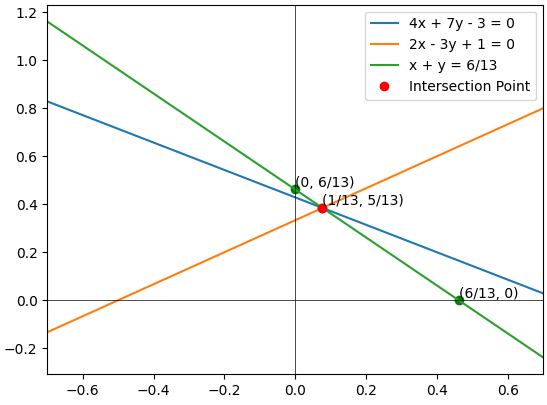
\includegraphics[width=\columnwidth]{chapters/11/10/4/12/figs/straightline.png}
    \caption{Straight Lines}
    \label{fig:enter-label}
\end{figure}
\end{enumerate}
